\documentclass[11pt,a4paper]{article}
\usepackage[margin=2.3cm]{geometry}
\usepackage{amsmath,amssymb}
\usepackage{graphicx}
\usepackage{booktabs}
\usepackage{array}
\usepackage{adjustbox}
\usepackage[hidelinks]{hyperref}
\emergencystretch=3em

\newcommand{\bu}{\boldsymbol{u}}
\newcommand{\bv}{\boldsymbol{v}}
\newcommand{\bw}{\boldsymbol{w}}
\newcommand{\bff}{\boldsymbol{f}}
\newcommand{\dt}{\Delta t}
\newcommand{\code}[1]{\texttt{#1}}

\title{Taylor--Hood $\theta$-schemes and adaptive SUPG\\for the time-dependent Navier--Stokes equations:\\implementation, observations and results}
\author{galerkit, branch \code{time-navier-stokes}}
\date{November 2026}

\begin{document}
\maketitle

\begin{abstract}
This report documents two pieces of code written on the galerkit branch \code{time-navier-stokes}
(package \code{galerkit.\allowbreak navier\_stokes.\allowbreak twod.\allowbreak theta\_th}).
Part~I is a fresh Taylor--Hood $P_2/P_1$ implementation of the coupled $\theta$-schemes of
John~\cite{John2016}, Sect.~7.3.1, without any stabilisation, together with the examples of that section
(Examples 7.44, 7.57 in two dimensions, 7.58 and 7.62, based on Examples D.5, D.7, D.8, D.9 of Appendix~D).
Part~II extends the adaptive SUPG method of de Frutos, Garc\'{\i}a-Archilla, John and Novo~\cite{FGJN14}
from evolutionary convection--diffusion--reaction equations to the Navier--Stokes equations, with the
inf-sup stable Taylor--Hood pair (no pressure stabilisation), and reports simulations for the smooth
solution of Example D.7 and for a manufactured solution with boundary layers of width $\sqrt\nu$.
All rates and comparisons below are \emph{observed numerically}; nothing in this report is a proof.
The verdict for Part~II: the implementation is verified; the direct extension of the FGJN14 error estimator is
robust globally but localises poorly, and its absolute local thresholds do not control the global error.
Adaptivity does not pay off on the smooth solution or for layers of width 0.01, but for layers of width 0.001
($\nu=10^{-6}$) the combination of an $h^1$-type indicator for the ranking, the FGJN14-type estimator for the
global error and D\"orfler marking beats uniform refinement (2.7--2.9 times smaller $L^2$ error with fewer
unknowns).
\end{abstract}

\tableofcontents

%======================================================================
\section{Common discretisation}
%======================================================================

We consider, in a bounded polygon $\Omega\subset\mathbb{R}^2$,
\begin{equation}\label{eq:nse}
\partial_t\bu-\nu\Delta\bu+(\bu\cdot\nabla)\bu+\nabla p=\bff,\qquad \nabla\cdot\bu=0,\qquad \bu(0)=\bu_0,
\end{equation}
with Dirichlet data on part of the boundary and, for the flows around a cylinder, the do-nothing condition
$\nu\partial_{\boldsymbol n}\bu-p\boldsymbol n=\boldsymbol 0$ at the outlet.

\paragraph{Space.} Continuous $P_2$ velocity and continuous $P_1$ pressure on triangles (Taylor--Hood).
Curved boundaries (the cylinder) are represented isoparametrically: every cell is mapped from the reference
triangle by the quadratic map defined by its six $P_2$ nodes, with edge midpoints on curved boundary parts placed
on the exact boundary. Integrals use a collapsed Gauss rule exact for polynomials of degree~7 on the reference
triangle. The viscous term is in gradient form, the convective term in convective form
$n(\bw,\bu,\bv)=((\bw\cdot\nabla)\bu,\bv)$ unless the skew-symmetric form
$\frac12[((\bw\cdot\nabla)\bu,\bv)-((\bw\cdot\nabla)\bv,\bu)]$ is stated.

\paragraph{Meshes.} Unit square: $2\times2$ squares, two triangles each with alternating diagonals, uniformly
refined; level $\ell$ has mesh width $h=\sqrt2\,2^{-(\ell+1)}$. Cylinder channel $(0,2.2)\times(0,0.41)$ minus the
disc of radius $0.05$ at $(0.2,0.2)$: a transfinite O-grid around the cylinder and a Cartesian block downstream,
split into triangles and refined uniformly; levels 1, 2, 3 have 5\,082, 19\,668, 77\,352 unknowns. The front and back
points of the cylinder are mesh vertices on every level.

\paragraph{Linear algebra.} Sparse direct solver: PARDISO (via \code{pypardiso}) when installed, SciPy's SuperLU
otherwise. PARDISO perturbs small pivots of the saddle-point matrices; every solve therefore checks
$\|b-Ax\|_2\le10^{-12}\|b\|_2$, refines iteratively up to three times with the cached factorisation and falls back
to SuperLU (Sect.~\ref{sec:pardiso}).

%======================================================================
\part{\texorpdfstring{$\theta$}{theta}-schemes after John (2016), Chapter 7}
%======================================================================

\section{Implementation}

Module \code{theta\_th.solver}, class \code{ThetaTH}. One substep from $t_k$ to $t_{k+1}=t_k+\dt_{k+1}$ inside the
macro step of length $\dt_{n+1}$ is the variational problem~\cite[(7.84)]{John2016}:
\begin{align*}
(\bu_{k+1},\bv)&+\theta_1\dt_{n+1}\big[\nu(\nabla\bu_{k+1},\nabla\bv)+n(\bu_{k+1},\bu_{k+1},\bv)\big]
-\dt_{k+1}(\nabla\cdot\bv,p_{k+1})\\
&=(\bu_k,\bv)-\theta_2\dt_{n+1}\big[\nu(\nabla\bu_k,\nabla\bv)+n(\bu_k,\bu_k,\bv)\big]
+\theta_3\dt_{n+1}(\bff_k,\bv)+\theta_4\dt_{n+1}(\bff_{k+1},\bv),\\
0&=\dt_{k+1}(\nabla\cdot\bu_{k+1},q),
\end{align*}
with the divergence constraint scaled by $\dt_{k+1}$ as in all simulations of~\cite{John2016} (Remark 7.50).
The book prints ``$2\nu$'' in the $\theta_2$ term of (7.84); (7.80)--(7.83) and (7.85) have $\nu$, which is used here.
The parameters $\theta_1,\dots,\theta_4$ are those of Tables 7.1 and 7.2 (module \code{theta\_th.schemes}):
backward Euler, Crank--Nicolson, the general one-step $\theta$-scheme, and the fractional-step schemes FS0 and FS1
with $\theta=1-\sqrt2/2$, $\tilde\theta=1-2\theta$, $\tau=\tilde\theta/(1-\theta)$, $\eta=1-\tau$.

Nonlinear solvers: Picard iteration (7.85) and Newton's method (7.86), initial iterate $(\bu_k,p_k)$, stopped when
the Euclidean norm of the residual of (7.84) on the non-Dirichlet rows is below $10^{-10}$; IMEX variants
(Remark 7.61) with the constant extrapolation $\bu_{\rm prev}=\bu_k$ or the linear extrapolation (7.89), the explicit
$\theta_2$ term using the convection field of the previous step as in (7.91).

\paragraph{Verification (unit tests, \code{tests/test\_ns2d\_theta\_th.py}).}
Tables 7.1/7.2 reproduced; stability functions $R(z)$ with $R(z)-e^z=O(z^{p+1})$, $R(-\infty)=-1$ (CN), $0$ (BE),
$-\eta/\tau\approx-0.71$ (FS0); exactness for a steady $P_2/P_1$ solution; time orders 1 (BE) and 2 (CN, FS0, FS1)
for a solution in the discrete space; IMEX orders 2 (linear) and 1 (constant extrapolation); quadratic convergence of
Newton's method.

\section{Example D.5: steady flow around a cylinder (validation)}

Re $=20$, inflow $1.2\,y(0.41-y)/0.41^2$, do-nothing outflow, drag and lift by the volume formulas (D.16), (D.17).

\begin{center}\begin{adjustbox}{max width=\textwidth}
\begin{tabular}{rrrrrr}
\toprule
level & unknowns & $c_d-c_{d,\rm ref}$ & $c_l-c_{l,\rm ref}$ & $\Delta p-\Delta p_{\rm ref}$ & Newton steps\\
\midrule
0 & 1\,353 & $+3.5\cdot10^{-2}$ & $+8.0\cdot10^{-2}$ & $+4.0\cdot10^{-3}$ & 5\\
1 & 5\,082 & $-9.7\cdot10^{-4}$ & $-5.2\cdot10^{-4}$ & $+6.1\cdot10^{-4}$ & 5\\
2 & 19\,668 & $-2.4\cdot10^{-4}$ & $-1.6\cdot10^{-4}$ & $+2.1\cdot10^{-4}$ & 5\\
3 & 77\,352 & $-1.7\cdot10^{-5}$ & $-1.2\cdot10^{-5}$ & $+5.9\cdot10^{-5}$ & 5\\
\bottomrule
\end{tabular}
\end{adjustbox}\end{center}
References (D.19), (D.21), (D.22): $c_d=5.57953523384$, $c_l=0.010618948146$ (do-nothing), $\Delta p=0.11752016697$.

\section{Example D.7: smooth solution, convergence}

$\Omega=(0,1)^2$, $\bu=2\pi\sin t\,(\sin^2(\pi x)\sin(\pi y)\cos(\pi y),\,-\sin(\pi x)\cos(\pi x)\sin^2(\pi y))$,
$p=20\sin t\,(x^2y-1/6)$, homogeneous Dirichlet data, $\nu=10^{-2}$, $T=1$.

\paragraph{Space} (FS0, $\dt=0.005$). The column ``$p$ shifted'' compares $p_h$ with $p$ at the time the last
substep's pressure approximates, $t_{k+1}-(1-\theta_1/(\theta_1+\theta_2))\dt_{k+1}$.
\begin{center}\begin{adjustbox}{max width=\textwidth}
\begin{tabular}{rllllllll}
\toprule
level & $\|\bu-\bu_h\|_0$ & rate & $\|\nabla(\bu-\bu_h)\|_0$ & rate & $\|p-p_h\|_0$ at $T$ & rate & $p$ shifted & rate\\
\midrule
0 & 4.30e-1 & & 6.34 & & 6.07e-1 & & 6.07e-1 &\\
1 & 1.31e-1 & 1.72 & 3.22 & 0.98 & 1.60e-1 & 1.93 & 1.59e-1 & 1.93\\
2 & 1.61e-2 & 3.02 & 0.822 & 1.97 & 2.81e-2 & 2.51 & 2.81e-2 & 2.51\\
3 & 1.98e-3 & 3.02 & 0.195 & 2.07 & 6.53e-3 & 2.11 & 6.39e-3 & 2.13\\
4 & 2.23e-4 & 3.15 & 0.0436 & 2.16 & 2.00e-3 & 1.71 & 1.52e-3 & 2.07\\
\bottomrule
\end{tabular}
\end{adjustbox}\end{center}
Observed: the optimal Taylor--Hood rates 3, 2, 2. The dip of the pressure rate at $T$ on level 4 is the first-order
temporal pressure error of FS0 at $t_{n+1}$; it disappears at the shifted time.

\paragraph{Time} (level 4). Velocity error at $T$ against the same scheme with $\dt=1/640$ on the same mesh (temporal
error only):
\begin{center}\begin{adjustbox}{max width=\textwidth}
\begin{tabular}{lllllllll}
\toprule
$\dt$ & BE & rate & CN & rate & FS0 & rate & FS1 & rate\\
\midrule
0.2 & 7.39e-2 & & 4.07e-3 & & 4.85e-4 & & 1.87e-3 &\\
0.1 & 3.65e-2 & 1.02 & 1.02e-3 & 2.00 & 1.20e-4 & 2.01 & 2.67e-4 & 2.81\\
0.05 & 1.80e-2 & 1.03 & 2.54e-4 & 2.00 & 3.00e-5 & 2.01 & 5.38e-5 & 2.31\\
0.025 & 8.68e-3 & 1.05 & 6.32e-5 & 2.00 & 7.47e-6 & 2.01 & 1.29e-5 & 2.06\\
0.0125 & 4.05e-3 & 1.10 & 1.56e-5 & 2.02 & 1.85e-6 & 2.02 & 3.10e-6 & 2.06\\
\bottomrule
\end{tabular}
\end{adjustbox}\end{center}
Observed: orders 1 (BE) and 2 (CN, FS0, FS1). Against the exact solution all second-order schemes level off at
$2.23\cdot10^{-4}$, the spatial error of level 4. The pressure is of first order at $t_{n+1}$ for every scheme
(Remark 7.50); the Crank--Nicolson pressure compared at $t_n+\dt/2$ converges with order 2 down to the spatial floor
$\approx1.5\cdot10^{-3}$; the FS0 pressure at $t_{n+1}-\eta\theta\dt$ is at the spatial floor already for $\dt=0.1$
(observed, no explanation proved); the FS1 pressure stays of first order there (plausibly because its last substep
evaluates $\bff$ only at the old time, $\theta_4=0$; not verified).

\section{Example 7.44: pressure error with Crank--Nicolson}

Book: $Q_2/P_1^{\rm disc}$, $\dt=10^{-4}$, $T=5$. Here: Taylor--Hood $P_2/P_1$, Crank--Nicolson with $\dt=10^{-3}$, $T=5$,
the discrete norm $\big(\dt\sum_n\|p(t)-p_h^n\|_0^2\big)^{1/2}$ with $p$ evaluated at $t_n$ or at $t_n-\dt/2$.

\begin{center}\begin{adjustbox}{max width=\textwidth}
\begin{tabular}{rllllllll}
\toprule
& \multicolumn{4}{c}{$\nu=1$} & \multicolumn{4}{c}{$\nu=10^{-2}$}\\
level & at $t_n$ & rate & at $t_n-\dt/2$ & rate & at $t_n$ & rate & at $t_n-\dt/2$ & rate\\
\midrule
0 & 1.65 & & 1.65 & & 1.25 & & 1.25 &\\
1 & 0.754 & 1.13 & 0.754 & 1.13 & 0.319 & 1.96 & 0.319 & 1.96\\
2 & 8.71e-2 & 3.11 & 8.71e-2 & 3.11 & 5.45e-2 & 2.55 & 5.44e-2 & 2.55\\
3 & 1.42e-2 & 2.62 & 1.39e-2 & 2.65 & 1.27e-2 & 2.10 & 1.24e-2 & 2.14\\
4 & 4.28e-3 & 1.73 & 3.01e-3 & 2.20 & 4.23e-3 & 1.59 & 2.94e-3 & 2.07\\
\bottomrule
\end{tabular}
\end{adjustbox}\end{center}
Observed (convective form): second order when the Crank--Nicolson pressure is compared at the midpoint, as in Fig.~7.2
of the book, and errors nearly independent of $\nu$ for $\nu\in\{1,10^{-2}\}$. Comparing at $t_n$ adds a temporal error
$\approx\frac{\dt}{2}\|\partial_tp\|$ that dominates on level 4.

For $\nu=10^{-4}$ the unstabilised scheme with the convective form blows up on level 1 ($\|\bu_h\|$ grows to 15 at
$t\approx2.5$, Newton then fails); the convective form is not energy stable for the only weakly divergence-free
Taylor--Hood velocity (plausible cause, not proved). With the skew-symmetric form the computation is stable, but the
pressure error stays large: 1.25, 7.18, 4.07, 3.85 on levels 0--3 (level 4 was not completed within the 2\,h limit
of the runs). The book's observation that the pressure error does not depend on $\nu$ does not hold for this
discretisation at $\nu=10^{-4}$ on these meshes.

\section{Example 7.57 in two dimensions: Picard iteration vs Newton's method}

The book's Example 7.57 is three-dimensional (Example D.10). Here: Example D.7, $\nu=10^{-3}$, Crank--Nicolson with
$\dt=0.01$ on $[0,0.1]$, solution of the previous time as initial iterate, stopping tolerance $10^{-10}$, direct solver.

\begin{center}\begin{adjustbox}{max width=\textwidth}
\begin{tabular}{rrlrrl}
\toprule
level & unknowns & method & linear systems (10 steps) & solve time [s] & $\|\bu(T)-\bu_h\|_0$\\
\midrule
2 & 659 & Picard & 29 & 0.27 & 2.406e-3\\
2 & 659 & Newton & 20 & 0.17 & 2.406e-3\\
3 & 2\,467 & Picard & 28 & 0.81 & 6.369e-4\\
3 & 2\,467 & Newton & 20 & 1.42 & 6.369e-4\\
4 & 9\,539 & Picard & 27 & 4.15 & 1.262e-4\\
4 & 9\,539 & Newton & 20 & 3.56 & 1.262e-4\\
5 & 37\,507 & Picard & 26 & 15.97 & 1.714e-5\\
5 & 37\,507 & Newton & 20 & 11.40 & 1.714e-5\\
\bottomrule
\end{tabular}
\end{adjustbox}\end{center}
As in Table 7.3 of the book, Newton's method needs fewer linear systems (two per step instead of about three). The
timings were taken on a shared machine and include the residual checks of the solver; they are indicative only.

\section{Example 7.58: flow around a cylinder with time-dependent inflow (Example D.9)}

$\nu=10^{-3}$, inflow $\sin(\pi t/8)\,6y(0.41-y)/0.41^2$ on $[0,8]$, $\bu_0=\boldsymbol0$, do-nothing outflow as in
Example 7.58, level 2 (19\,668 unknowns), Newton's method, tolerance $10^{-10}$. The book uses $Q_2/P_1^{\rm disc}$ on
levels 3--5 (37\,216 to 588\,160 unknowns).

\begin{center}\begin{adjustbox}{max width=\textwidth}
\begin{tabular}{lrrrrrr}
\toprule
scheme, $\dt$ & $c_{d,\max}$ & $t$ & $c_{l,\max}$ & $t$ & $\Delta p(8)$ & linear solves\\
\midrule
BE, 0.02 & 2.950769 & 3.9320 & 0.001159 & -- & $-0.126729$ & 800\\
BE, 0.01 & 2.950513 & 3.9319 & 0.023069 & 7.3443 & $-0.124637$ & 1\,600\\
BE, 0.005 & 2.950404 & 3.9320 & 0.166381 & 6.3505 & $-0.107584$ & 3\,200\\
CN, 0.02 & 2.950700 & 3.9418 & 0.444633 & 5.7997 & $-0.098212$ & 948\\
CN, 0.01 & 2.950758 & 3.9382 & 0.462118 & 5.7615 & $-0.103691$ & 1\,754\\
CN, 0.005 & 2.950771 & 3.9363 & 0.466132 & 5.7508 & $-0.105762$ & 3\,200\\
FS0, 0.02 & 2.950792 & 3.9362 & 0.464448 & 5.7539 & $-0.105187$ & 2\,413\\
FS0, 0.01 & 2.950784 & 3.9352 & 0.466521 & 5.7483 & $-0.106273$ & 4\,466\\
FS0, 0.005 & 2.950778 & 3.9347 & 0.466880 & 5.7466 & $-0.106606$ & 7\,257\\
\midrule
Table D.3 & 2.950918381 & 3.93625 & 0.47787543 & 5.69250 & $-0.11161567$ &\\
\bottomrule
\end{tabular}
\end{adjustbox}\end{center}
Table D.3 was computed with the Dirichlet outflow (D.29) on fine meshes; the remaining gap of $c_{l,\max}$ is mostly
spatial. Errors (discrete $l^2(0,8)$) to the FS0 run with $\dt=0.005$ on the same mesh (temporal errors only):

\begin{center}\begin{adjustbox}{max width=\textwidth}
\begin{tabular}{lllll}
\toprule
scheme, $\dt$ & $c_d$ & $c_l$ & $\Delta p$ & linear solves\\
\midrule
BE, 0.005 & 1.14e-1 & 4.05e-1 & 6.24e-2 & 3\,200\\
CN, 0.02 & 1.91e-2 & 2.95e-1 & 2.27e-2 & 948\\
CN, 0.01 & 8.13e-3 & 8.61e-2 & 9.24e-3 & 1\,754\\
CN, 0.005 & 3.39e-3 & 2.41e-2 & 3.66e-3 & 3\,200\\
FS0, 0.02 & 3.48e-3 & 4.23e-2 & 4.07e-3 & 2\,413\\
FS0, 0.01 & 1.10e-3 & 9.69e-3 & 1.22e-3 & 4\,466\\
\bottomrule
\end{tabular}
\end{adjustbox}\end{center}
Observed, as in the book: backward Euler is by far the least accurate and misses the vortex shedding for
$\dt\ge0.005$ (Fig.~\ref{fig:d9}, cf.\ Fig.~7.5); Crank--Nicolson converges with order about two; FS0 is 5--9 times more
accurate than Crank--Nicolson at equal $\dt$ and still 2--2.5 times more accurate at comparable cost (the reference is
FS0 itself, which favours FS0; against a Crank--Nicolson reference the ordering is the same). The book reports a slightly
better accuracy per CPU time for Crank--Nicolson (Remark 7.59, John and Rang 2010); that is not reproduced here, which
depends on the solver.

\begin{figure}[ht]
\centering
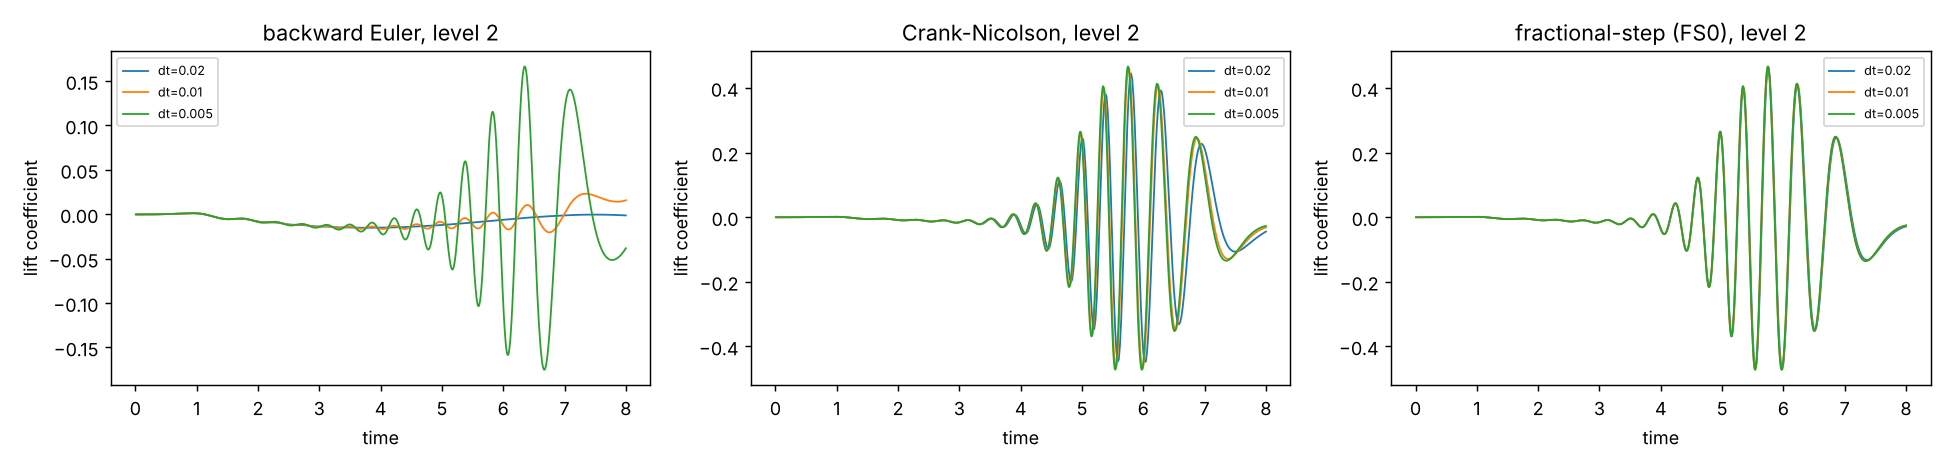
\includegraphics[width=\textwidth]{figures/d9_L2_lift.png}\\[1ex]
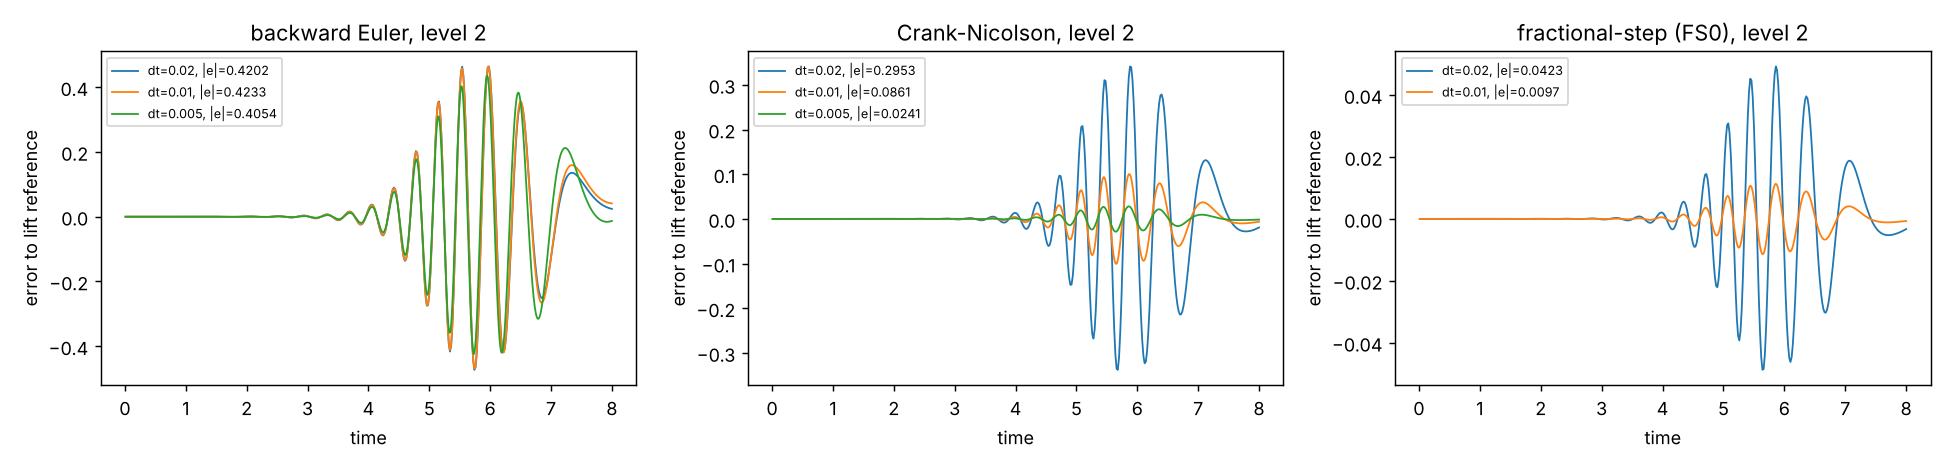
\includegraphics[width=\textwidth]{figures/d9_L2_error_lift.png}
\caption{Example 7.58 / D.9, level 2: lift coefficient (top) and its error to the FS0 run with $\dt=0.005$ (bottom).}
\label{fig:d9}
\end{figure}

\section{Example 7.62: IMEX schemes (Example D.8)}

Re $=100$, steady inflow $6y(0.41-y)/0.41^2$, spin-up with Crank--Nicolson ($\dt=0.01$) to $t=15$, then two time units
with Crank--Nicolson, $\dt=0.005$, level 2.
\begin{center}\begin{adjustbox}{max width=\textwidth}
\begin{tabular}{lrrrrr}
\toprule
method & $c_{d,\max}$ & $c_{l,\max}$ & St & $\Delta p(t_0+T/2)$ & linear solves\\
\midrule
fully implicit (Newton) & 3.2222 & 0.9841 & 0.2984 & 2.4858 & 800\\
IMEX, linear extrapolation & 3.2341 & 1.0052 & 0.3008 & 2.4930 & 400\\
IMEX, constant extrapolation & 3.4010 & 1.5833 & 0.2857 & 2.5892 & 400\\
\midrule
Table D.2 & [3.22, 3.24] & [0.98, 1.02] & [0.295, 0.305] & [2.46, 2.50] &\\
\bottomrule
\end{tabular}
\end{adjustbox}\end{center}
Observed, as in Fig.~7.10: the constant extrapolation is quite inaccurate (and its amplitude still grows), the linear
extrapolation gives almost the same results as the fully implicit scheme with half the linear solves; both lie inside
all four reference intervals on level 2. On level 1 (5\,082 unknowns) the flow is not resolved (St $\approx0.27$).

\begin{figure}[ht]
\centering
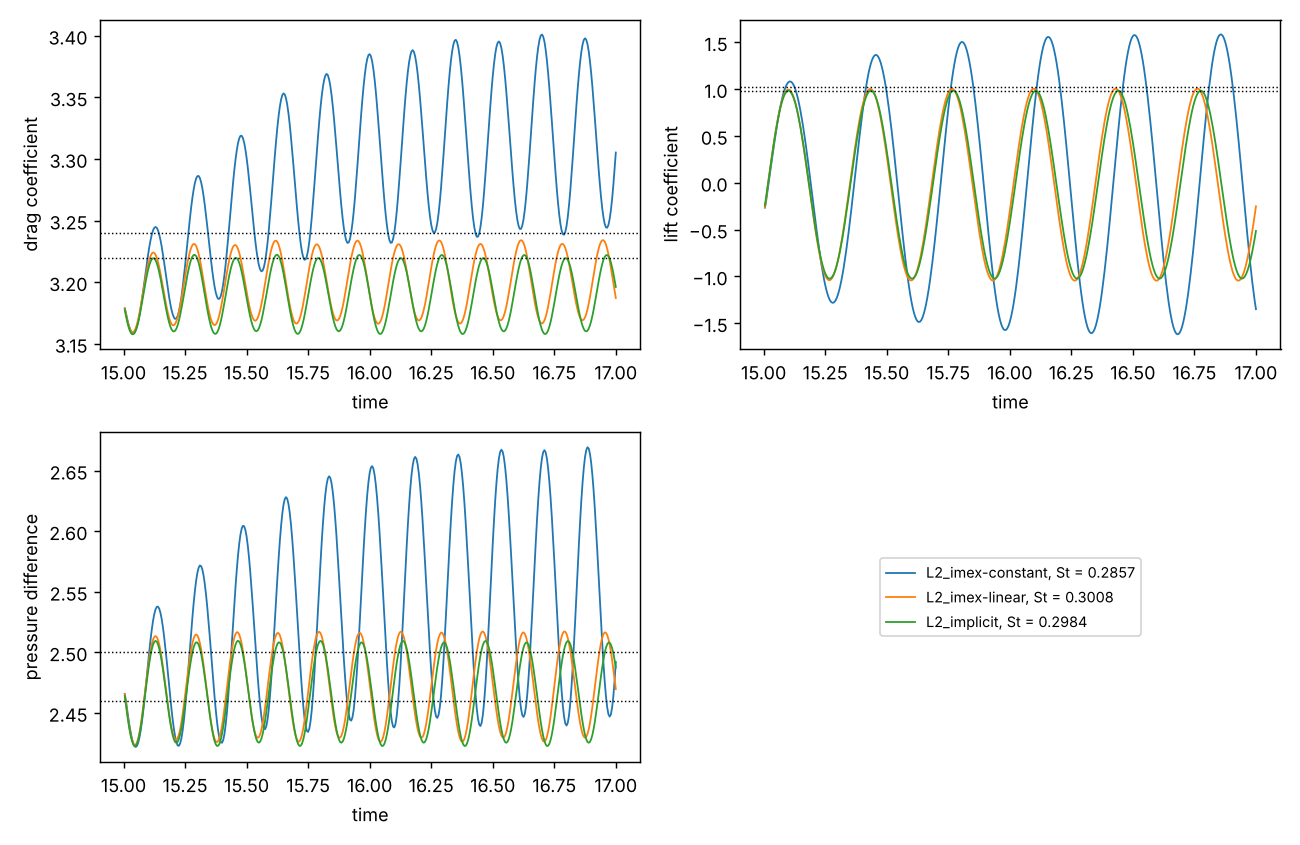
\includegraphics[width=0.85\textwidth]{figures/d8_L2_qoi.png}
\caption{Example 7.62 / D.8, level 2: drag, lift and pressure difference; dotted: reference intervals of Table D.2.}
\end{figure}

%======================================================================
\part{Adaptive SUPG for Navier--Stokes (extension of FGJN14)}
%======================================================================

\section{Discretisation}

Module \code{theta\_th.supg}, class \code{SUPGTH}. With the transport field $\bw=\bu_h$ (fully nonlinear) and the
discrete time derivative $\bu_h'$,
\begin{multline*}
(\bu_h',\bv)+\nu(\nabla\bu_h,\nabla\bv)+((\bw\cdot\nabla)\bu_h,\bv)-(p_h,\nabla\cdot\bv)\\
+\sum_K\delta_K\big(\bu_h'-\nu\Delta\bu_h+(\bw\cdot\nabla)\bu_h+\nabla p_h-\bff,(\bw\cdot\nabla)\bv\big)_K=(\bff,\bv),
\qquad(\nabla\cdot\bu_h,q)=0.
\end{multline*}
The pressure gradient is part of the consistent residual; there is \emph{no} pressure stabilisation (no PSPG, no
grad-div): Taylor--Hood is inf-sup stable. Time: the trapezoidal rule with the discrete derivative as in~\cite{FGJN14},
Sect.~3.3, $\bu_{n+1}=\bu_n+\frac{\dt}2(\bu_n'+\bu_{n+1}')$, the equation collocated at $t_{n+1}$; with $\delta_K=0$ this
is algebraically Crank--Nicolson (reproduced to all digits). Stabilisation parameter (a choice of this implementation;
\cite{FGJN14} use $\delta_0h_K/\|\boldsymbol b\|_{\infty,K}$):
\[
\delta_K=\delta_0\min\big\{h_K/\|\bw_0\|_{\infty,K},\,h_K^2/\nu\big\},\qquad\delta_0=0.25,
\]
computed from the initial iterate $\bw_0=\bu_n+\dt\,\bu_n'$ of the step and kept fixed in the nonlinear iteration.
Newton's method with the full Jacobian (Galerkin convection and both SUPG derivatives
$\delta_K((\delta\bu\cdot\nabla)\bu,(\bu\cdot\nabla)\bv)$ and $\delta_K(R(\bu),(\delta\bu\cdot\nabla)\bv)$), an Armijo line
search and a Picard fallback. Stopping criterion: $\|r\|_2\le10^{-10}$ for the residual with the momentum rows scaled by
$\dt/2$ (velocity units, independent of $\dt$). A first version used the unscaled residual with a relative tolerance;
because of the factor $2/\dt\approx10^{10}$ for tiny steps it accepted unsolved iterates (found with the boundary-layer
problem, Sect.~\ref{sec:layers}).

\paragraph{Verification (\code{tests/test\_ns2d\_adaptive\_supg\_th.py}).} A steady $P_2/P_1$ solution is reproduced to
round-off for $\delta_0\in\{0,0.25,5\}$ (consistency); Newton's method converges quadratically; the transfer between
meshes is exact under refinement; all residuals vanish for a discrete solution.

\section{Adaptive algorithm}

Module \code{theta\_th.adaptive}, class \code{AdaptiveSUPGNS}, following the steps of~\cite{FGJN14}, Sect.~3.3, as
implemented for convection--diffusion in \code{galerkit.convection\_diffusion.adaptive\_supg} (the PDF of~\cite{FGJN14}
was not at hand; details of its p.~227 not covered there may differ). After every accepted time step:
\begin{enumerate}
\item TR step; step size by the TR-AB2 controller of Gresho, Griffiths and Silvester: AB2 predictor,
  $d=(\bu-\bu^p)/(3(1+\dt_{\rm old}/\dt))$ in the $L^2$ norm of the velocity, $\dt_{\rm new}=0.85\dt({\rm tol}_t/\|d\|)^{1/3}$,
  rejection if $\|d\|>{\rm tol}_t/0.7^3$, averaging every 10 steps, $\dt_0=10^{-10}$;
\item local indicators $\eta_K$ (an \code{ErrorIndicator});
\item marking (a \code{Marking}): FGJN14 thresholds ($\eta_K>{\rm TOL}_1$ refine, $\eta_K<{\rm TOL}_2={\rm TOL}_1/20$ coarsen) or
  D\"orfler marking (below);
\item newest-vertex bisection and its exact inverse;
\item transfer of $\bu_h$ by interpolation (exact under refinement).
\end{enumerate}
Additions needed for Navier--Stokes (each documented in the code with the failure it prevents):
(i) after a mesh change $\bu_h'$ and $p_h$ are recomputed from the discrete equation (an interpolated $\bu_h'$ violates it
by $O(1)$; 325 rejections in 4 accepted steps were observed); (ii) the step may grow by at most a factor 10 (from
$\dt_0=10^{-10}$ the predictor is exact and the unlimited formula proposed $\dt\approx10^{88}$); (iii) the nonlinear
iteration starts from the predictor, and a failed step is repeated with $\dt/2$; (iv) $\delta_K$ is computed from the
predictor ($\bu(0)=\boldsymbol0$ in Example D.7 gave $\delta_K=\delta_0h^2/\nu\approx80$ otherwise).
Three further additions were found with the boundary-layer problem of Sect.~\ref{sec:layers}, where $\bu_0\neq\boldsymbol0$:
(v) the initial velocity and every velocity transferred to a new mesh are $L^2$-projected onto the discretely
divergence-free subspace (the $P_2$ interpolant of $\bu_0$ has $\|B\bu_0\|=0.046$; the first TR step then projects it, a
jump independent of $\dt$ that the TR-AB2 estimate rejects for every step size, and the run stalled at
$\dt\approx10^{-10}$); (vi) the $\dt$-independent stopping criterion of the previous section; (vii) the initial mesh is
adapted to $\bu_0$, by refinement only, until the global estimate of $\bu_0$ is below the target of the marking (errors
made on a too coarse initial mesh are carried along at small $\nu$ and are not removed by later refinement; with only 8
initial passes the global error stalled at $3.9\cdot10^{-2}$ on 47\,000 cells, and with coarsening allowed the initial
passes cycled between 80 and 82 cells).

\paragraph{Marking.} Besides the FGJN14 thresholds, \code{DoerflerMarking}: if the global estimate (of the marking
indicator or of a separate \code{global\_indicator}) exceeds a target, refine the smallest set of cells carrying the
fraction $\theta$ of $\sum_K m_K^2$; cells carrying together the smallest fraction of $\sum_Km_K^2$ (default 5\,\%, 0 = no
coarsening) are coarsening candidates. It uses only the ranking of $m_K$.

\paragraph{Error indicators, designed to be extended.} All residual indicators share
\[
R_K=\bff-\bu_h'+\nu\Delta\bu_h-(\bu_h\cdot\nabla)\bu_h-\nabla p_h,\qquad
R_E=-\nu[\![\partial_{\boldsymbol n}\bu_h]\!],\qquad R_{\rm div}=\nabla\cdot\bu_h,
\]
and differ in their weights (a \code{Weights} subclass):
\[
\eta_K^2=w_K\|R_K\|_K^2+\sum_{E\subset\partial K}w_E\|R_E\|_E^2+w_{{\rm div},K}\|\nabla\cdot\bu_h\|_K^2 .
\]
\begin{center}\begin{adjustbox}{max width=\textwidth}
\begin{tabular}{lll}
\toprule
name & weights & origin\\
\midrule
\code{supg} & $w_K=\min\{h_K^2/\nu,24\delta_K\}+24\delta_K$, $w_E=\min\{24/\|\bu_h\|_{\infty,E},h_E/\nu\}$, $w_{\rm div}=\nu$
& \cite[(28)]{FGJN14}, $\varepsilon\to\nu$, $\boldsymbol b\to\bu_h$, $c\to0$\\
\code{h1} & $h_K^2$, $h_E$, $1$ & energy-norm weights\\
\code{l2} & $h_K^4$, $h_E^3$, $h_K^2$ & $L^2$ weights\\
\code{exact} & local SUPG-norm error of a known solution & for testing\\
\code{exact\_l2} & local $L^2$ velocity error of a known solution & for testing\\
\bottomrule
\end{tabular}
\end{adjustbox}\end{center}
The divergence term is an addition of this extension (Taylor--Hood is only weakly divergence free). A new indicator is a
new \code{Weights} or \code{ErrorIndicator} subclass registered in \code{INDICATORS}; the marking strategy is exchangeable
as well, and a separate \code{global\_indicator} may supply the global estimate.

\section{Results for the smooth solution (Example D.7)}

$T=1$, $\delta_0=0.25$, ${\rm tol}_t=10^{-3}$, initial mesh $4\times4$ squares. Error measures at $T$: $\|\bu-\bu_h\|_0$ and
the SUPG norm $(\nu|\bu-\bu_h|_1^2+\sum_K\delta_K\|(\bu_h\cdot\nabla)(\bu-\bu_h)\|_K^2)^{1/2}$.

\subsection{Uniform meshes and effectivity}

\begin{center}\begin{adjustbox}{max width=\textwidth}
\begin{tabular}{llll}
\toprule
$\nu$, method & $\|\bu-\bu_h\|_0$, levels 1$\to$4 & rates & SUPG norm, levels 1$\to$4\\
\midrule
$10^{-2}$, SUPG & 1.22e-1 $\to$ 7.73e-4 & 2.47, 2.50, 2.34 & 6.56e-1 $\to$ 2.11e-2 (rates 1.66, 1.62, 1.68)\\
$10^{-2}$, Galerkin & 1.31e-1 $\to$ 2.24e-4 & 3.02, 3.02, 3.15 & --\\
$10^{-4}$, SUPG & 1.60e-1 $\to$ 7.75e-3 & 0.92, 1.39, 2.06 & 6.94e-1 $\to$ 4.75e-2 (rates 1.26, 1.31, 1.30)\\
$10^{-4}$, Galerkin & 3.05e-1 $\to$ 3.98e-3 & 1.41, 2.08, 2.77 & --\\
\bottomrule
\end{tabular}
\end{adjustbox}\end{center}
(Unknowns on levels 1--4: 188, 660, 2\,468, 9\,540. The ``SUPG norm'' of a Galerkin run lacks the $\delta$ term and is not
listed.) On these meshes SUPG is less accurate than Galerkin in $L^2$ for this resolved smooth solution, and its SUPG-norm
rates (1.3--1.7) are below the $h^{k+1/2}=h^{2.5}$ of the theory for convection-dominated problems; whether this is
pre-asymptotic or an effect of the choice of $\delta_K$ is open.

Effectivity $\eta/\|e\|_{\rm SUPG}$ on uniform meshes (levels 1--4, after 20 steps of $\dt=0.01$):
\begin{center}\begin{adjustbox}{max width=\textwidth}
\begin{tabular}{llll}
\toprule
$\nu$ & \code{supg} & \code{h1} & \code{l2}\\
\midrule
$10^{-2}$ & 11.6, 13.4, 15.6, 17.7 & 5.4, 7.0, 8.0, 8.7 & 1.9, 1.2, 0.7, 0.4\\
$10^{-4}$ & 10.0, 8.2, 8.5, 9.1 & 6.7, 12.9, 24.5, 41.2 & 2.4, 2.3, 2.2, 1.8\\
\bottomrule
\end{tabular}
\end{adjustbox}\end{center}
The extended FGJN14 estimator is robust in $\nu$ (as reported in~\cite{FGJN14} for convection--diffusion), the \code{h1}
weights are not.

\subsection{Adaptive runs}

The table shows the runs with all additions (i)--(vii) (re-run after the boundary-layer study; the uniform, effectivity and
time-adaptivity results did not change).
\begin{center}\begin{adjustbox}{max width=\textwidth}
\begin{tabular}{llrrrlll}
\toprule
$\nu$ & marking & cells & unknowns & steps (rej.) & $\|\bu-\bu_h\|_0$ & SUPG norm & max Newton\\
\midrule
$10^{-2}$ & \code{supg}, TOL$_1$ 0.04 & 478 & 2\,300 & 45 (0) & 5.88e-3 & 7.65e-2 & 3\\
$10^{-2}$ & \code{supg}, TOL$_1$ 0.02 & 866 & 4\,131 & 44 (0) & 3.10e-3 & 4.68e-2 & 3\\
$10^{-2}$ & \code{supg}, TOL$_1$ 0.01 & 1\,594 & 7\,457 & 41 (0) & 1.36e-3 & 2.60e-2 & 3\\
$10^{-2}$ & \code{exact}, TOL$_1$ 5e-3 / 2.5e-3 / 1.25e-3 & 525 / 771 / 1\,181 & 2\,484 / 3\,606 / 5\,466 & 53 / 49 / 44 (0) & 4.95e-3 / 2.60e-3 / 1.65e-3 & 6.07e-2 / 3.66e-2 / 2.75e-2 & 3\\
\midrule
$10^{-4}$ & \code{supg}, TOL$_1$ 0.04 & 697 & 3\,338 & 54 (3) & 4.50e-2 & 1.59e-1 & 22\\
$10^{-4}$ & \code{supg}, TOL$_1$ 0.02 & 1\,451 & 6\,806 & 63 (2) & 2.23e-2 & 1.20e-1 & 9\\
$10^{-4}$ & \code{supg}, TOL$_1$ 0.01 & 2\,142 & 10\,048 & 48 (1) & 1.41e-2 & 6.71e-2 & 15\\
$10^{-4}$ & \code{exact}, TOL$_1$ 5e-3 & 1\,092 & 5\,083 & 55 (0) & 2.10e-2 & 8.27e-2 & 3\\
$10^{-4}$ & \code{exact}, TOL$_1$ 2.5e-3 & 2\,066 & 9\,541 & 45 (0) & 1.22e-2 & 5.14e-2 & 4\\
$10^{-4}$ & \code{exact}, TOL$_1$ 1.25e-3 & 4\,514 & 20\,597 & 45 (0) & 8.60e-3 & 3.14e-2 & 4\\
$10^{-4}$ & D\"orfler, \code{h1}/\code{supg}, 0.5 & 975 & 4\,589 & 59 (0) & 2.77e-2 & 1.36e-1 & 3\\
$10^{-4}$ & D\"orfler, \code{h1}/\code{supg}, 0.3 & 2\,880 & 13\,344 & 67 (0) & 1.29e-2 & 7.27e-2 & 3\\
$10^{-4}$ & D\"orfler, \code{h1}/\code{supg}, 0.2 & 3\,918 & 18\,025 & 63 (0) & 9.86e-3 & 4.83e-2 & 3\\
\midrule
$10^{-4}$ & uniform level 4 & 2\,048 & 9\,540 & 100 ($\dt=0.01$) & 7.75e-3 & 4.75e-2 & 3\\
\bottomrule
\end{tabular}
\end{adjustbox}\end{center}
D\"orfler marking here: $\theta=0.3$, 5\,\% coarsening. Compared with the first version (before additions (v)--(vii)), the
same tolerances give smaller meshes for $\nu=10^{-4}$, at about the same or slightly better accuracy per unknown; with the
\code{supg} thresholds the errors now decrease monotonically with TOL$_1$ (before: SUPG norm 8.3e-2, 9.6e-2, 5.9e-2 on
9\,560, 10\,270, 18\,738 unknowns), and the maximal number of Newton iterations dropped from 30 to 22. A plausible
explanation, not verified: before addition (v) every transferred velocity carried a spurious divergence residual that
inflated the estimators right after each mesh change and triggered extra refinement. For $\nu=10^{-2}$ the results are
practically unchanged.

\begin{figure}[ht]
\centering
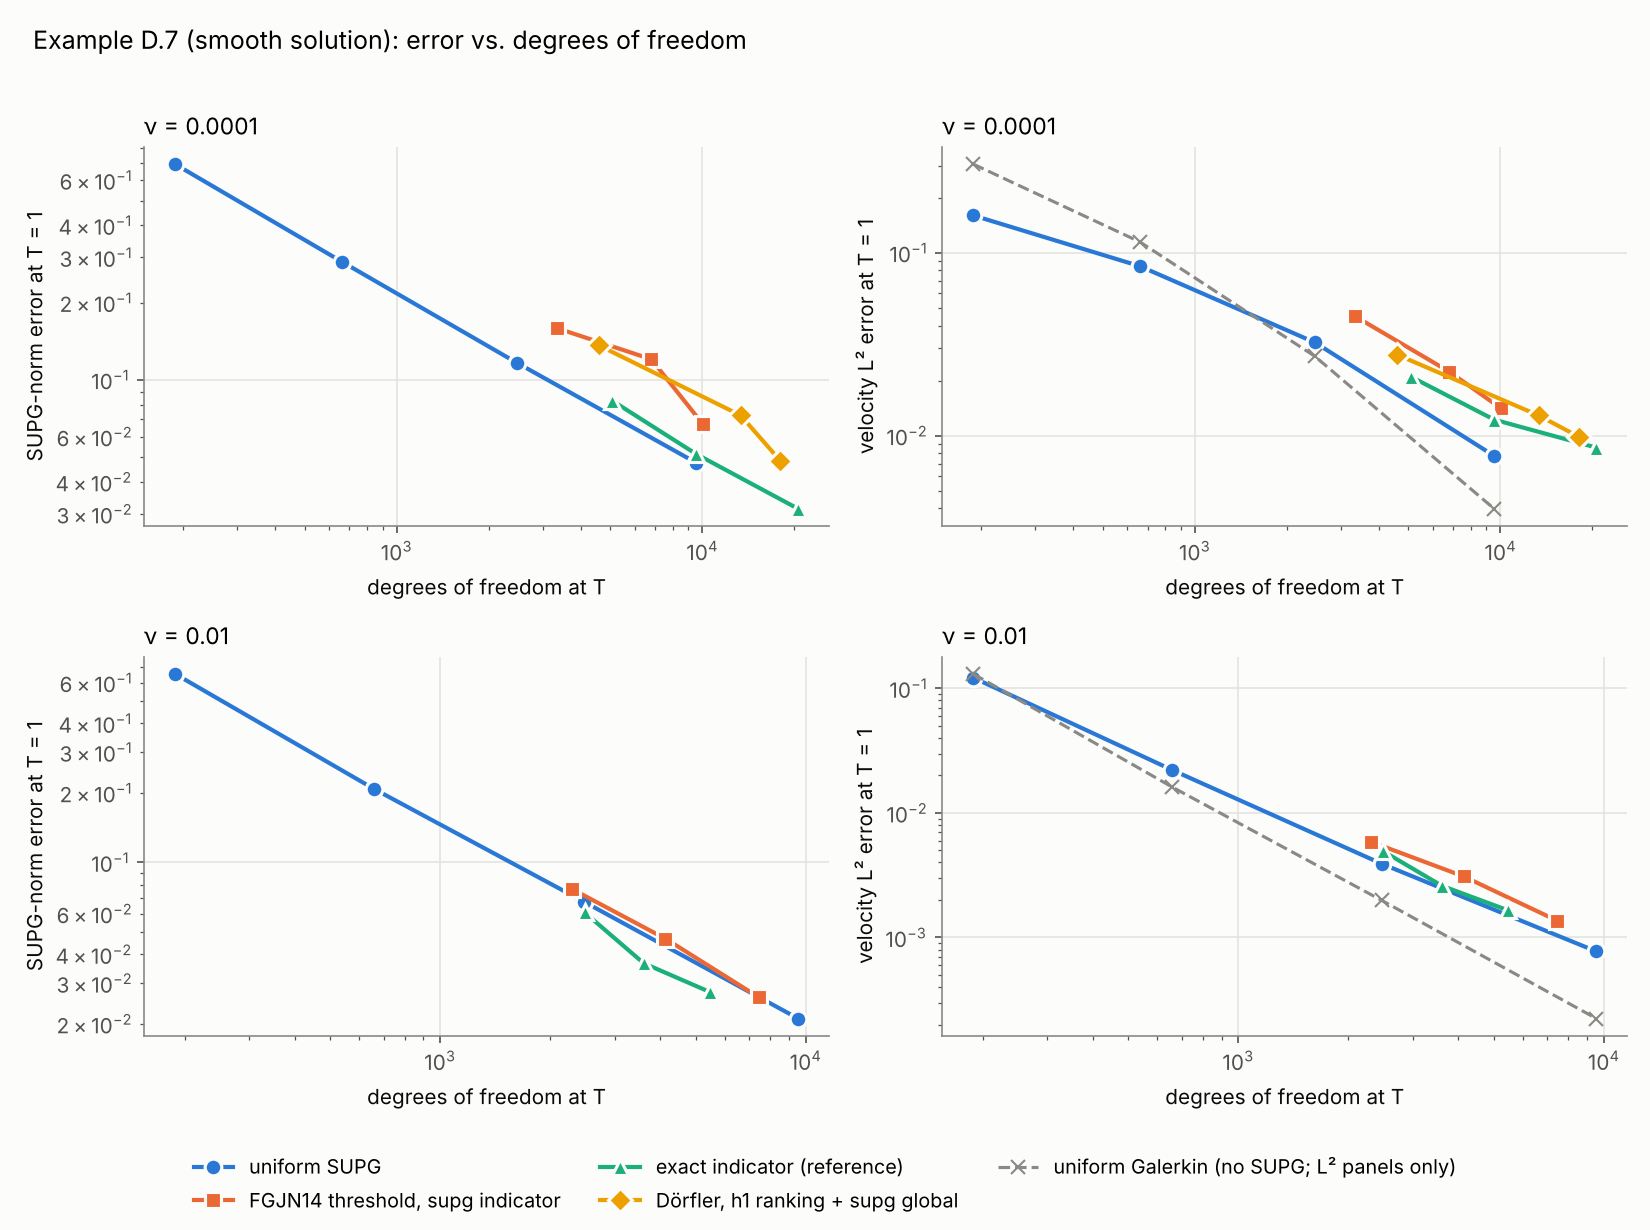
\includegraphics[width=\textwidth]{figures/adaptive_error_vs_dofs.png}
\caption{Example D.7: error at $T=1$ against the number of unknowns ($\nu=10^{-4}$ top, $10^{-2}$ bottom).}
\label{fig:adaptive}
\end{figure}

\begin{figure}[ht]
\centering
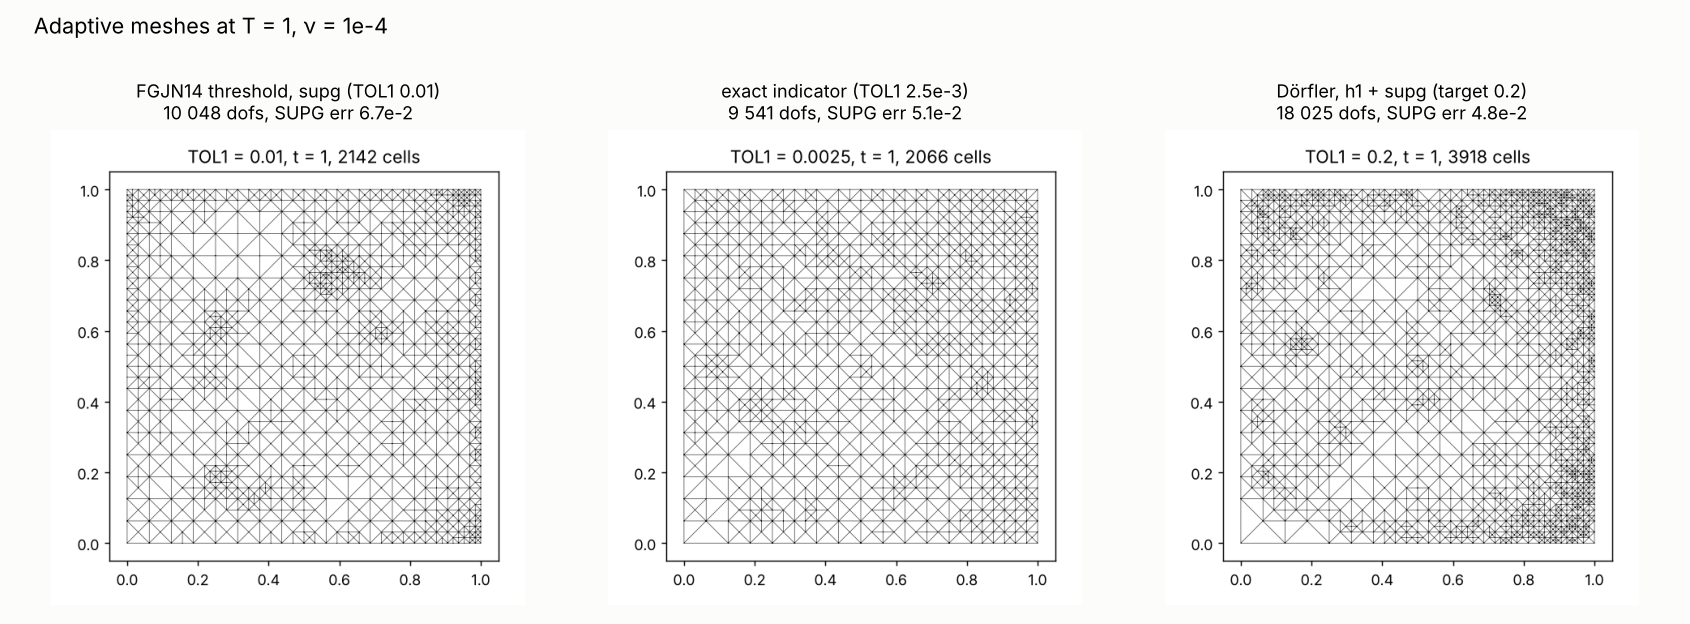
\includegraphics[width=\textwidth]{figures/adaptive_meshes_nu1e-4.png}
\caption{Adaptive meshes at $T=1$, $\nu=10^{-4}$.}
\end{figure}

\subsection{Diagnosis of the \code{supg} indicator}

On the same SUPG states (uniform levels 3, 4, $t=0.5$) $\eta_K$ was compared cell by cell with the exact local SUPG-norm
error $e_K$ (\code{diagnose\_indicator.py}). For $\nu=10^{-4}$, level 4:
\begin{center}\begin{adjustbox}{max width=\textwidth}
\begin{tabular}{lllll}
\toprule
weights & effectivity & Spearman($\eta_K,e_K$) & top-10\,\% overlap & slow cells' share of $\eta^2$ (of $e^2$: 0.39)\\
\midrule
\code{supg} & 6.6 & 0.41 & 0.62 & 0.85\\
\code{supg}, $\delta_K$ capped at $\delta_0h_K/U_\infty$ & 2.5 & 0.47 & 0.67 & 0.65\\
cell weight $h_K^2$, \code{supg} edge & 1.7 & 0.66 & 0.74 & 0.89\\
edge + divergence terms only & 1.7 & 0.70 & 0.74 & 0.89\\
\code{h1} & 36.8 & 0.79 & 0.79 & 0.71\\
\bottomrule
\end{tabular}
\end{adjustbox}\end{center}
(``slow'': $\|\bu_h\|_{\infty,K}<0.2$.) For $\nu=10^{-2}$, level 4: \code{supg} effectivity 14.7, Spearman 0.51, top-10\,\%
overlap 0.21; \code{h1} 7.95, 0.97, 0.76. At $\nu=10^{-4}$ the cell part of $\eta^2$ is 37--41 times $\sum e_K^2$, the edge
part 0.2--2.7 times, the divergence part at most 0.14 times.

\begin{figure}[ht]
\centering
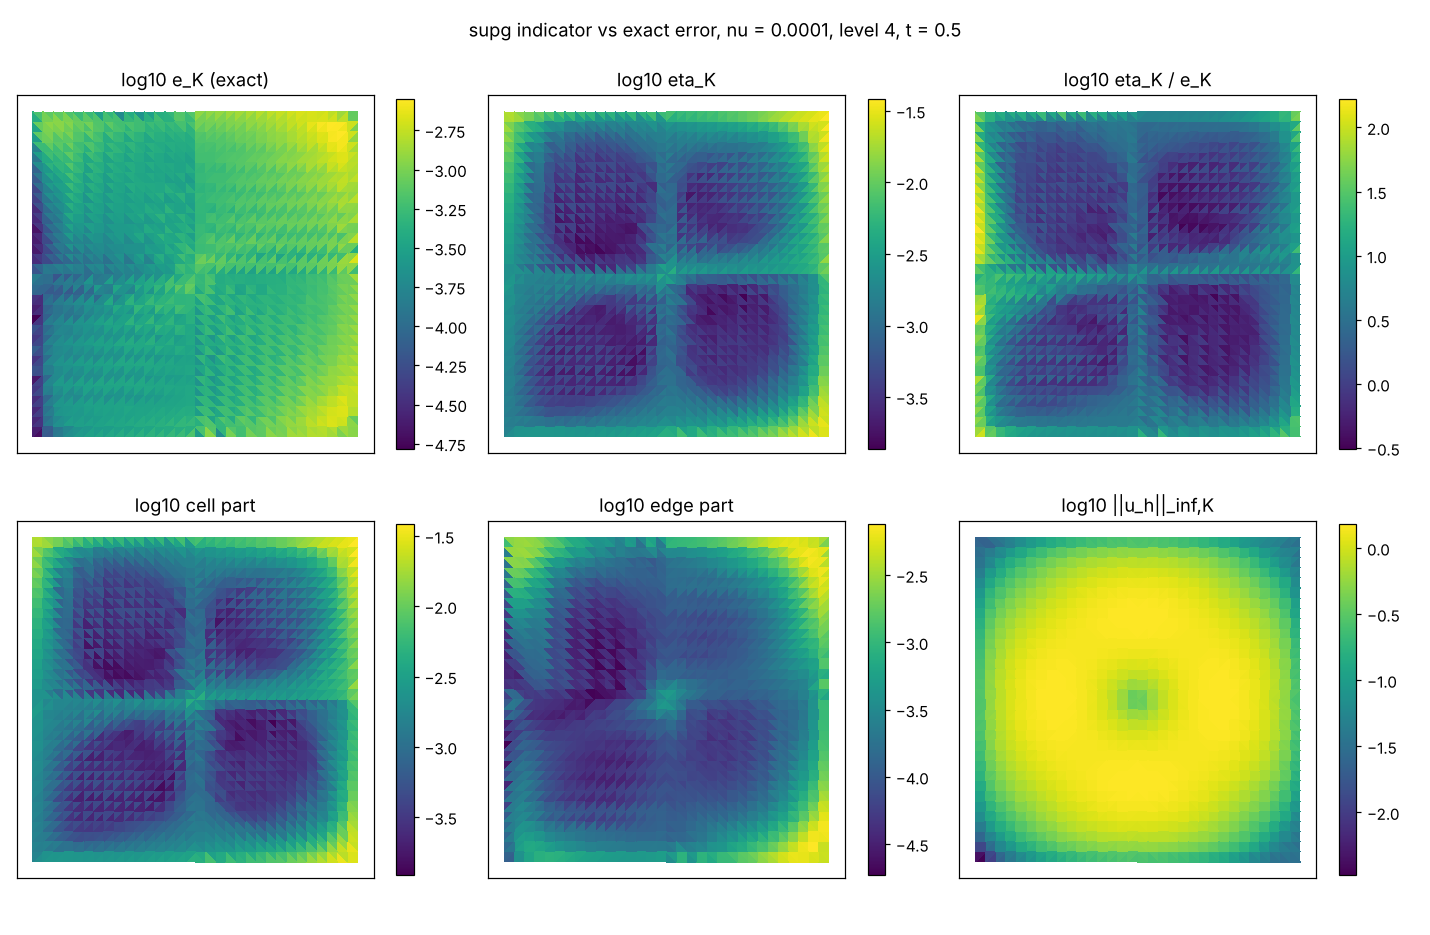
\includegraphics[width=\textwidth]{figures/diagnosis_maps_nu1e-4_L4.png}
\caption{$\nu=10^{-4}$, level 4, $t=0.5$: exact local error, \code{supg} indicator, their ratio, cell and edge parts,
local velocity (all $\log_{10}$).}
\end{figure}

\section{Results for boundary layers of width \texorpdfstring{$\sqrt\nu$}{sqrt(nu)}}\label{sec:layers}

Problem (\code{problems.BoundaryLayer}; the \code{LayerSolution} of galerkit branch \code{kelvin-helmholtz}, ported, $\bff$
checked against SymPy to $5\cdot10^{-15}$): in $(0,1)^2$, with $\delta=\sqrt\nu$ and $g(t)=1+\frac12\sin(2\pi t)$,
\begin{gather*}
L(y)=(1-e^{-y/\delta})(1-e^{-(1-y)/\delta}),\quad m=\int_0^1L,\quad a(y)=L(y)-6my(1-y),\quad Y(y)=\int_0^ya,\\
\bu=g(t)\big(\sin^2(\pi x)\,a(y),\,-\pi\sin(2\pi x)\,Y(y)\big),\qquad p=g(t)\cos(\pi x)\cos(\pi y).
\end{gather*}
$\bu=\boldsymbol0$ on the whole boundary, $\nabla\cdot\bu=0$; $u_1$ rises from 0 to $O(1)$ within $O(\delta)$ of $y=0$ and
$y=1$, the interior flow is a shear that changes sign; $\bff$ is $O(1)$ uniformly in $\nu$. Settings: $T=0.25$,
${\rm tol}_t=10^{-4}$, $\delta_0=0.25$, initial mesh $4\times4$, initial adaptation to $\bu_0$ (addition (vii)); uniform
runs with $\dt=0.005$.

\paragraph{$\nu=10^{-4}$ (layers 0.01 wide).}
\begin{center}\begin{adjustbox}{max width=\textwidth}
\begin{tabular}{lrrll}
\toprule
method & unknowns at $T$ & max cells & $\|\bu-\bu_h\|_0$ & SUPG norm\\
\midrule
uniform SUPG, level 3 / 4 / 5 / 6 & 2\,468 / 9\,540 / 37\,508 / 148\,740 & -- & 4.49e-2 / 1.15e-2 / 1.95e-3 / 2.84e-4 & 8.53e-2 / 3.27e-2 / 1.08e-2 / 3.27e-3\\
uniform Galerkin, level 4 / 5 / 6 & 9\,540 / 37\,508 / 148\,740 & -- & 1.14e-2 / 1.85e-3 / 2.44e-4 & --\\
\code{exact} + D\"orfler ($\theta=0.3$, 5\,\% coarsening), target 0.03 & 20\,285 & 10\,901 & 1.26e-2 & 2.95e-2\\
\code{exact} + D\"orfler, target 0.015 & 33\,566 & 11\,073 & 5.75e-3 & 1.42e-2\\
\code{exact} + D\"orfler, no coarsening, target 0.03 & 14\,857 & 3\,199 & 1.01e-2 & 2.87e-2\\
\code{h1}/\code{supg} D\"orfler, target 0.2 / 0.1 / 0.05 & 14\,290 / 27\,336 / 62\,061 & 7\,797 / 9\,272 / 16\,353 & 8.80e-3 / 3.24e-3 / 1.55e-3 & 3.58e-2 / 1.66e-2 / 9.79e-3\\
FGJN14 thresholds, \code{supg}, TOL$_1$ 0.02 / 0.01 & 5\,456 / 9\,731 & 1\,181 / 2\,179 & 1.47e-2 / 5.62e-3 & 5.33e-2 / 3.09e-2\\
\bottomrule
\end{tabular}
\end{adjustbox}\end{center}
No adaptive variant beats uniform refinement in the SUPG norm, also not with the exact indicator; the only gain is in
$L^2$ for the FGJN14 thresholds (5.6e-3 against 1.15e-2 at $\approx9\,600$ unknowns). With FGJN14 thresholds even the exact
indicator was worse than uniform (TOL$_1=2\cdot10^{-3}$: $L^2$ error $3.7\cdot10^{-2}$ on 19\,823 unknowns at $T=0.25$):
with an absolute local tolerance many coarse interior cells each stay just below TOL$_1$ and add up to a large global
error. The 5\,\% coarsening in every step made the D\"orfler mesh oscillate (coarsening pushes the error above the target,
D\"orfler refines 30\,\% back); without coarsening the same accuracy needs at most 3\,199 instead of 10\,901 cells (31\,s
instead of 365\,s), but is still slightly worse than uniform ($\approx2.3\cdot10^{-2}$ at 14\,857 unknowns, interpolated).
Plausible reason (not verified): at $\nu=10^{-4}$ the layers are not thin compared with the scales of the $O(1)$ interior
shear, which needs a fairly fine mesh everywhere; uniform level 5 ($h\approx0.022$) already resolves the layers reasonably.

\begin{figure}[ht]
\centering
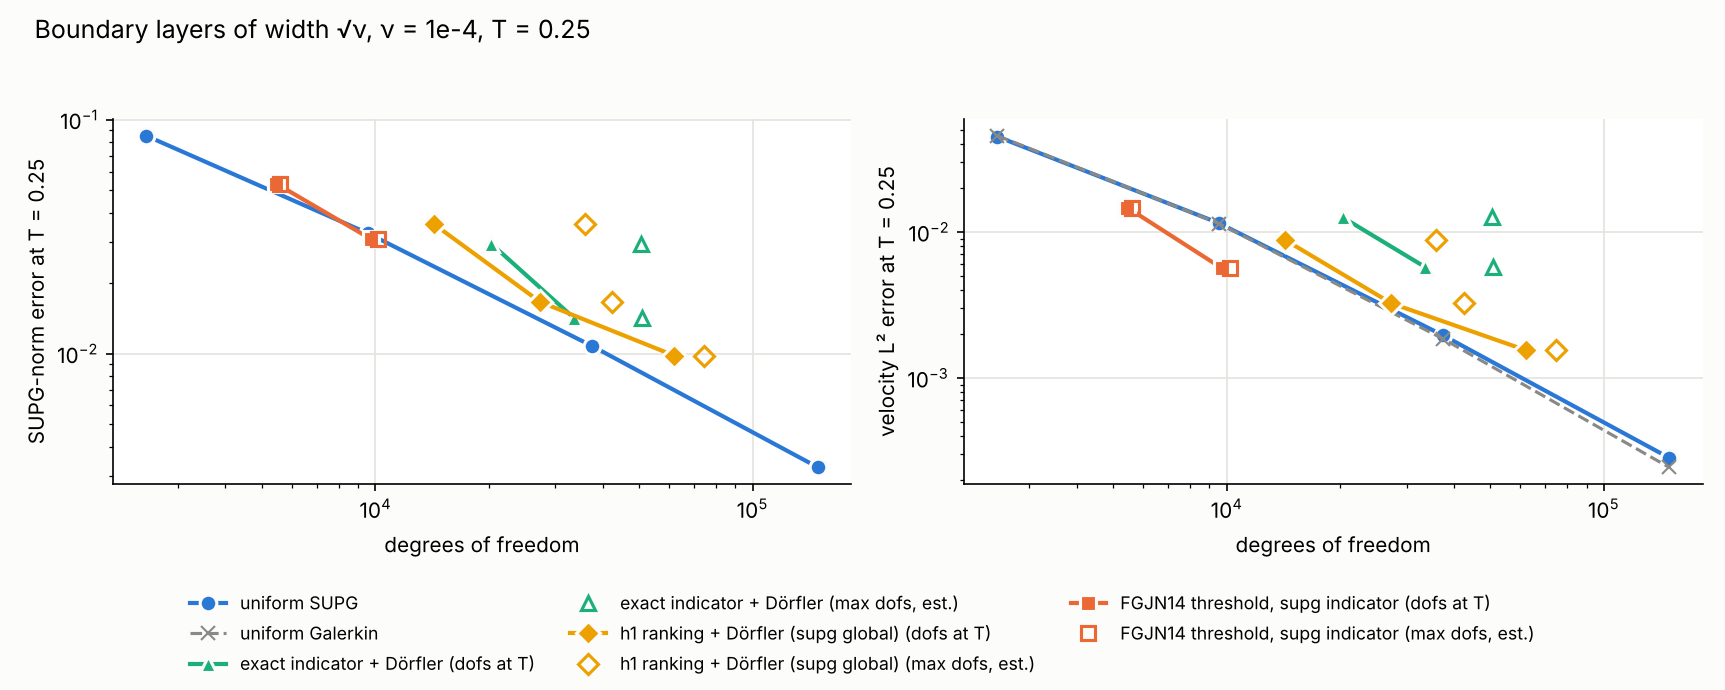
\includegraphics[width=\textwidth]{figures/layer_nu1e-4_error_vs_dofs.png}
\caption{Boundary layers, $\nu=10^{-4}$, $T=0.25$: error against unknowns (filled: at $T$; hollow: estimated maximum
during the run).}
\end{figure}

\paragraph{$\nu=10^{-6}$ (layers 0.001 wide).} D\"orfler marking without coarsening, maximal refinement level 22.
\begin{center}\begin{adjustbox}{max width=\textwidth}
\begin{tabular}{lrll}
\toprule
method & unknowns at $T$ (= max) & $\|\bu-\bu_h\|_0$ & SUPG norm\\
\midrule
uniform SUPG, level 4 / 5 / 6 & 9\,540 / 37\,508 / 148\,740 & 8.00e-2 / 4.74e-2 / 2.19e-2 & 6.40e-2 / 3.77e-2 / 2.19e-2\\
uniform Galerkin, level 6 & 148\,740 & 2.21e-2 & --\\
\textbf{\code{h1}/\code{supg} D\"orfler, target 0.1} & \textbf{62\,381} & \textbf{8.08e-3} & \textbf{2.00e-2}\\
\textbf{\code{h1}/\code{supg} D\"orfler, target 0.05} & \textbf{114\,167} & \textbf{7.68e-3} & \textbf{1.62e-2}\\
\code{exact} + D\"orfler, target 0.02 & 239\,866 & 4.16e-2 & 1.99e-2\\
\code{exact} + D\"orfler, target 0.01 & 319\,909 & 5.36e-3 & 7.99e-3\\
FGJN14 thresholds, \code{supg}, TOL$_1$ 0.01 & 12\,338 & 4.20e-2 & 4.36e-2\\
\bottomrule
\end{tabular}
\end{adjustbox}\end{center}
Here adaptivity pays off: \code{h1} ranking + D\"orfler with the \code{supg} global estimate has, compared with uniform
level 6, a 2.7 times smaller $L^2$ error and a slightly smaller SUPG-norm error with 42\,\% of the unknowns (target 0.1),
and a 2.9 times smaller $L^2$ error and a 1.35 times smaller SUPG-norm error with 77\,\% of the unknowns (target 0.05).
Uniform refinement converges slowly ($L^2$ rates 0.76 and 1.1 between levels 4--5--6; level 6 has $h\approx11\delta$). The
exact SUPG-norm indicator needs a much tighter target before it resolves the layer (at 0.02 its $L^2$ error is still
$4.2\cdot10^{-2}$; at 0.01 it is the most accurate run, with 320\,000 unknowns): at $\nu=10^{-6}$ the SUPG norm is dominated
by $10^{-3}|e|_1$ and is weak for an unresolved layer. The FGJN14 thresholds with \code{supg} are cheap but inaccurate.
Not completed (killed by the out-of-memory killer at $\approx14$\,GB): uniform level 7 and the exact $L^2$ indicator with
targets 0.02 and 0.01, whose meshes grew without bound (a plausible reason, not verified: $L^2$ error created in the
layers is convected into the interior, and refining where it sits does not remove it). The levels 4 and 5 of the uniform
run were transcribed from its log because the run was killed before writing its result file.

\begin{figure}[ht]
\centering
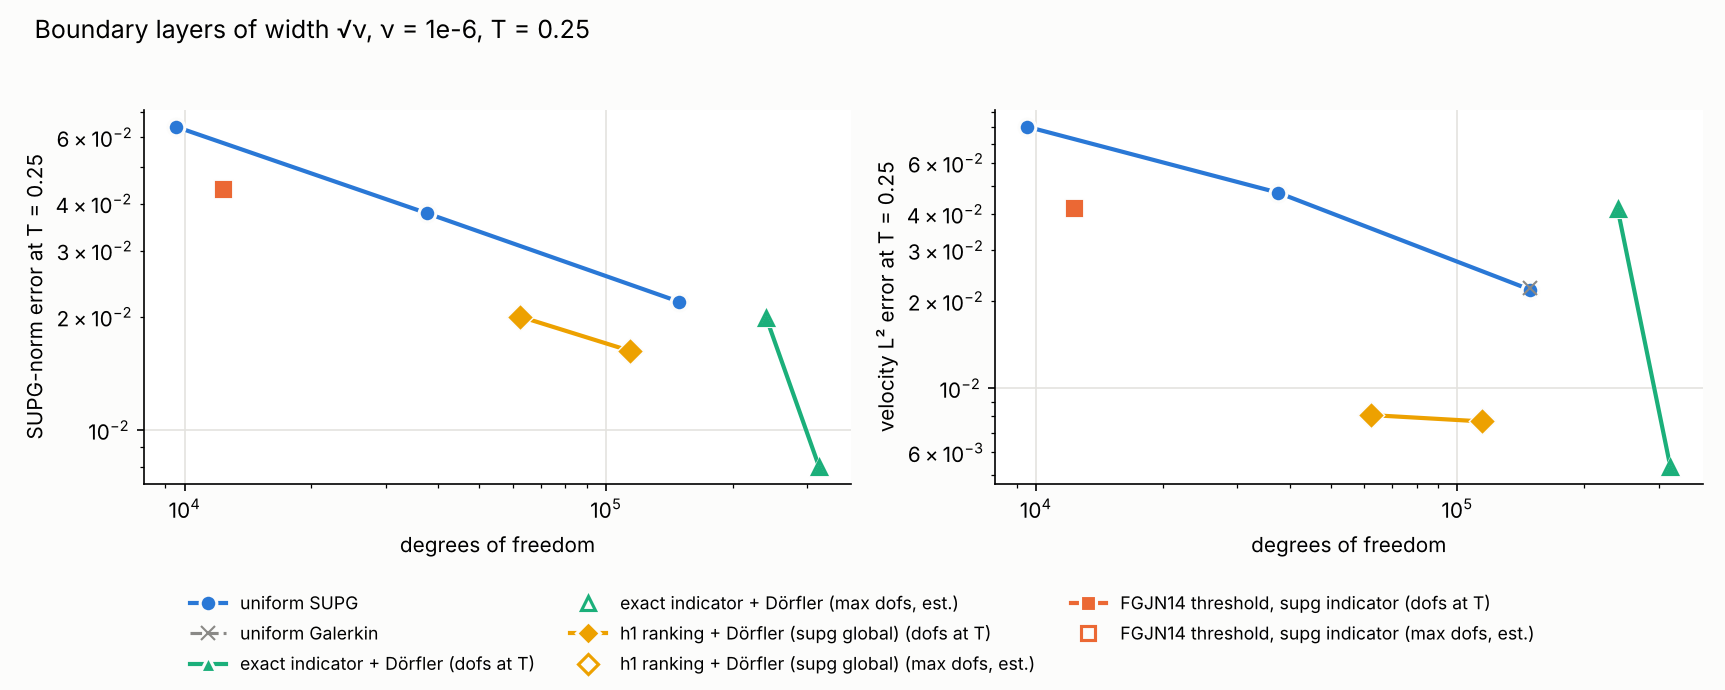
\includegraphics[width=\textwidth]{figures/layer_nu1e-6_error_vs_dofs.png}
\caption{Boundary layers, $\nu=10^{-6}$, $T=0.25$: error against unknowns.}
\end{figure}

\section{Observations}

\begin{enumerate}
\item \textbf{The cell weight of the extended FGJN14 estimator is unbounded where $\bu_h\to0$.} With
  $\delta_K=\delta_0h_K/\|\bu_h\|_{\infty,K}$ the weight $\min\{h_K^2/\nu,24\delta_K\}+24\delta_K\approx48\delta_K$ grows like
  $h_K/|\bu_h|$; $\delta_K/h_K$ reaches 65 near walls and vortex centres. In~\cite{FGJN14} the convection $\boldsymbol b$ is
  given and typically bounded away from zero; in Navier--Stokes it is not. At $\nu=10^{-4}$, level 4, cells with
  $\|\bu_h\|_{\infty,K}<0.05$ carry 44\,\% of $\eta^2$ and 5.5\,\% of $e^2$. The estimator is robust globally but ranks the
  cells poorly; this explains its poor adaptive meshes (up to 22 Newton iterations; before addition (v) also errors that
  were not monotone in TOL$_1$ and up to 30 Newton iterations).
\item \textbf{Marking and global estimate must be separated.} The \code{h1} indicator ranks the cells best but its magnitude
  is not robust in $\nu$; with D\"orfler marking on \code{h1} and the \code{supg} global estimate the adaptive runs at
  $\nu=10^{-4}$ behave as intended (monotone errors, no rejections, at most 7 Newton iterations). The control run with
  D\"orfler marking on \code{supg} collapsed: its 5\,\% ``smallest'' cells are the fast-flow cells, where the error is; the
  mesh was coarsened there (157 $\to$ 45 cells), the error grew from 0.15 to 0.28, the estimate exploded to $\sim10^5$ and the
  step size to $\sim10^{-10}$ near $t=0.414$.
\item \textbf{Adaptivity pays off only for thin layers.} On the smooth solution (D.7) no variant is more efficient than
  uniform refinement (the exact indicator at $\nu=10^{-4}$: $5.1\cdot10^{-2}$ on 9\,541 unknowns against $4.75\cdot10^{-2}$ on
  9\,540 for uniform level 4); for layers of width 0.01 ($\nu=10^{-4}$) neither, also not with the exact indicator. For
  layers of width 0.001 ($\nu=10^{-6}$) \code{h1} ranking + D\"orfler with the \code{supg} global estimate beats uniform
  level 6 in both norms with fewer unknowns (Sect.~\ref{sec:layers}).
\item \textbf{Absolute local thresholds do not control the global error} when the error is unevenly distributed: many cells
  just below TOL$_1$ add up (boundary layers, $\nu=10^{-4}$: the exact indicator with FGJN14 thresholds had a 3.2 times larger
  $L^2$ error than uniform level 4 with about twice its unknowns). D\"orfler marking with a global target does; its coarsening must be
  gentle or switched off, otherwise the mesh oscillates.
\item \textbf{Time-error floor not settled.} On D.7 the time-adaptivity study shows no influence of ${\rm tol}_t$ between
  $10^{-2}$ and $10^{-4}$ on level 3 (spatial error dominant); whether the slowly decreasing adaptive $L^2$ errors at
  $\nu=10^{-4}$ (Fig.~\ref{fig:adaptive}) are limited by ${\rm tol}_t=10^{-3}$ was not tested.
\item \textbf{SUPG vs Galerkin.} For this resolved smooth solution SUPG is less accurate than Galerkin in $L^2$
  on uniform meshes, and its SUPG-norm rates are below theory; open (pre-asymptotic behaviour or the choice of $\delta_K$).
\end{enumerate}

\section{A solver artefact: inaccurate PARDISO solves}\label{sec:pardiso}

With PARDISO, the adaptive run with the exact indicator and TOL$_1=1.25\cdot10^{-3}$, executed as the third run in one
process, ended with a SUPG-norm error of 0.20 instead of 0.029; the error jumped tenfold in the last steps. With SuperLU,
the same sequence gives 0.029 (identical to a standalone run), and the first two runs agree to all printed digits. On the
mass/divergence saddle-point system solved after each mesh change, PARDISO's relative residual was $8.5\cdot10^{-10}$
against $2\cdot10^{-14}$ for SuperLU. The residual-checked solve (iterative refinement, SuperLU fallback) restores the
SuperLU result exactly; in that run 54 refinements and one fallback occurred in 589 solves. Which mechanism inside PARDISO
(pivot perturbation or reused state) causes the inaccuracy was not established. With \code{pypardiso} installed, six
existing tests of older galerkit modules also fail (precision), independently of this work.

\section{Summary}

Part~I reproduces the qualitative findings of~\cite{John2016}, Sect.~7.3.1, with Taylor--Hood $P_2/P_1$: optimal spatial
rates for the smooth solution, temporal orders 1/2/2/2 for BE/CN/FS0/FS1, the pressure time levels of Remark~7.50, the
inaccuracy of backward Euler and the higher accuracy of FS0 for the flow around a cylinder, Newton needing fewer linear
systems than Picard, and the IMEX results of Example~7.62. Deviations: the element, coarser meshes, and the failure of the
unstabilised scheme at $\nu=10^{-4}$ in Example~7.44.

Part~II gives a verified SUPG--Taylor--Hood discretisation with the trapezoidal rule and an adaptive algorithm with
exchangeable indicators and marking strategies, extending~\cite{FGJN14} to Navier--Stokes; seven additions to the
algorithm were needed, each prompted by an observed failure. The direct extension of the FGJN14 estimator is robust
globally but localises poorly, because its cell weight is unbounded where the velocity vanishes, and absolute local
thresholds do not control the global error. With \code{h1} ranking, the \code{supg} estimator as global measure and
D\"orfler marking without coarsening, adaptivity beats uniform refinement for boundary layers of width 0.001
($\nu=10^{-6}$): 2.7--2.9 times smaller $L^2$ error with 42--77\,\% of the unknowns of uniform level 6. It does not pay off
on the smooth solution or for layers of width 0.01. Open: a cell weight that stays bounded for $\bu_h\to0$ (needs
analysis), the moving-layer case (time adaptivity), finer uniform references and other end times for $\nu=10^{-6}$.

\paragraph{Reproduction.} {\sloppy Code and scripts: galerkit, branch \code{time-navier-stokes},
\code{examples/\allowbreak navier\_stokes/\allowbreak 2d/\allowbreak theta\_john2016} (\code{d5\_steady.py}, \code{d7\_convergence.py}, \code{picard\_newton.py},
\code{d9\_cylinder.py}, \code{d8\_imex.py}) and \code{examples/\allowbreak navier\_stokes/\allowbreak 2d/\allowbreak adaptive\_supg\_ns} (\code{adaptive\_d7.py},
\code{diagnose\_indicator.py}, \code{plot\_summary.py}, \code{plot\_layer.py}); each script has \code{--smoke} and documents its options.\par}

\begin{thebibliography}{9}
\bibitem{John2016} V.~John, \emph{Finite Element Methods for Incompressible Flow Problems}, Springer Series in
Computational Mathematics 51, Springer, 2016.
\bibitem{FGJN14} J.~de Frutos, B.~Garc\'{\i}a-Archilla, V.~John, J.~Novo, An adaptive SUPG method for evolutionary
convection--diffusion equations, \emph{Comput. Methods Appl. Mech. Engrg.} 273 (2014) 219--237.
\end{thebibliography}

\end{document}
